\documentclass[11pt, addpoints, answers]{exam}

\usepackage{amsmath, amssymb}
\usepackage{xcolor}
\usepackage{drawstack}
\usepackage{physics}

\newcommand{\red}[1]{\textcolor{red}{#1}}

% For inserting code snippets.
\usepackage{listings}
\lstset{
    columns = fixed,
    basewidth = {0.5em},
    breaklines = true,
    backgroundcolor = \color{white},
    keywordstyle = \color[RGB]{40, 40, 255},
    numberstyle = \footnotesize\color{darkgray},
    commentstyle = \ttfamily\color{violet},
    basicstyle = \ttfamily,
    stringstyle = \ttfamily\color[RGB]{128, 0, 0},
    showstringspaces = false,
    language = {[11]C++},
    escapechar = \@
}
\lstnewenvironment{cpp}[1][]{\lstset{language = {[11]C++}, #1}}{}

\usepackage{tikz}
\usepackage{algorithmicx}

% headers, footers, titles
\newcommand{\CourseName}{CS101 Algorithms and Data Structures}
\newcommand{\HomeworkNO}{Homework 9}
\newcommand{\DueDate}{Due date: December 18, 2023, at 23:59}

\pagestyle{headandfoot}
\runningheadrule
\runningheader{\CourseName}{\HomeworkNO}{\DueDate}
\runningfooter{}{\thepage}{}

\title{
    \CourseName\\
    Fall 2023\\
    \HomeworkNO
}
\author{}
\date{\DueDate}

% formats of questions, choices, points, etc.
\qformat{\textbf\thequestion. (\totalpoints\ points) \thequestiontitle\hfill}
\pointname{'}
\CorrectChoiceEmphasis{\color{blue}}
\SolutionEmphasis{\color{blue}}

% We frequently use this font.
\newcommand{\ttt}{\texttt}
\newcommand{\bluett}[1]{\textcolor{blue}{\ttt{#1}}}

\begin{document}

    \maketitle

    \begin{enumerate}
        \item Please write your solutions in English.
        \item Submit your solutions to gradescope.com.
        \item Set your FULL name to your Chinese name and your STUDENT ID correctly in Account Settings.
        \item If you want to submit a handwritten version, scan it clearly. \ttt{CamScanner} is recommended.
        \item When submitting, match your solutions to the problems correctly.
        \item No late submission will be accepted.
        \item Violations to any of the above may result in zero points.
    \end{enumerate}

    \begin{questions}

        \newpage

        \titledquestion{Multiple Choices}

Each question has \textbf{one or more} correct answer(s). Select all the correct answer(s). For each question, you will get 0 points if you select one or more wrong answers, but you will get 1 point if you select a non-empty subset of the correct answers.

Write your answers in the following table.

%%%%%%%%%%%%%%%%%%%%%%%%%%%%%%%%%%%%%%%%%%%%%%%%%%%%%%%%%%%%%%%%%%%%%%%%%%%
% Note: The `LaTeX' way to answer a multiple-choices question is to replace `\choice'
% with `\CorrectChoice', as what you did in the first question. However, there are still
% many students who would like to handwrite their homework. To make TA's work easier,
% you have to fill your selected choices in the table below, no matter whether you use 
% LaTeX or not.
%%%%%%%%%%%%%%%%%%%%%%%%%%%%%%%%%%%%%%%%%%%%%%%%%%%%%%%%%%%%%%%%%%%%%%%%%%%

\begin{table}[htbp]
    \centering
    \begin{tabular}{|p{2cm}|p{2cm}|p{2cm}|p{2cm}|p{2cm}|p{2cm}|}
        \hline
        (a) & (b) & (c) & (d) & (e) & (f) \\
        \hline
        %%%%%%%%%%%%%%%%%%%%%%%%%%%%%%%%%%%%%%%%%%%%%%%%%%%%%%%%%%
        % YOUR ANSWER HERE.
        &     &     &     &     &     \\
        %%%%%%%%%%%%%%%%%%%%%%%%%%%%%%%%%%%%%%%%%%%%%%%%%%%%%%%%%%
        \hline
    \end{tabular}\label{tab:multiple}
\end{table}

\begin{parts}
    \part[2] Which of the following statements is/are true about \textbf{tree}?

    \begin{choices}
        \choice A tree with $N$ nodes has $N-1$ edges.
        \choice The height of a tree is always positive.
        \choice Every node of a tree is either a leaf node or an internal node.
        \choice The degree and the depth of the root node should be $0$.
    \end{choices}

    \part[2] Which of the following statements is/are true about \textbf{binary tree}?

    \begin{choices}
        \choice In a binary tree, every non-root node has exactly one parent.
        \choice Every full binary tree is also a complete binary tree.
        \choice A full binary tree with $n$ non-leaf nodes contains $2n - 1$ total nodes.
        \choice A binary tree of height $0$ is also perfect.
    \end{choices}

    \part[2] Which of the following choices is/are $\Theta(m)$ where $m$ is the maximum length of the queue when traversing a tree with BFS?

    \begin{choices}
        \choice The total number of nodes in the tree.
        \choice The length of the deepest path from a leaf node to the root node.
        \choice The maximum degree of nodes in the tree.
        \choice The maximum number of nodes at a given depth of the tree.
    \end{choices}

    \part[2] There exists two paths between any two different nodes in a tree with height more than 3.

    \begin{choices}
        \choice True.
        \choice False.
    \end{choices}

    \part[2] The height of a tree is always equal to the maximum depth of nodes in the tree.

    \begin{choices}
        \choice True.
        \choice False.
    \end{choices}

    \part[2] Which of the following statements is/are false?

    \begin{choices}
        \choice Nodes with the same depth are siblings.
        \choice Each node in the tree has exactly one parent pointing to it.
        \choice Given any node $\alpha$ within a tree, the collection of $\alpha$ and all of its descendants is a subtree of the tree with root $\alpha$.
        \choice The root node cannot be the descendent of any nodes.
    \end{choices}

\end{parts}

        \newpage

        \titledquestion{Topological Sort}

Given the following DAG, run topological sort with a queue. Write down the vertex you select and update the in-degree \texttt{ind[i]} of all vertices in each iteration.

\textit{Note: When pushing several vertices into the queue at the same time, push them alphabetically. You are NOT required to show your queue at each step.}

\vspace{1cm}

\begin{figure}[htbp]
    \centering
    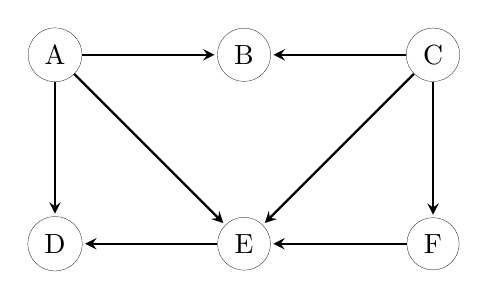
\begin{tikzpicture}[
        > = stealth, % arrow head style
        shorten > = 1pt, % don't touch arrow head to node
        node distance = 1cm, % distance between nodes
        thick, % line style
        scale = 0.8,
    ]
        % Draw the nodes
        \foreach \pos/\i in {
            (-3,3)/A,
            (0,3)/B,
            (3,3)/C,
            (-3,0)/D,
            (0,0)/E,
            (3,0)/F} {
            \node[circle, draw, line width=0.1pt] (\i) at \pos {\i};
        }

        % Draw the edges
        \foreach \b/\e in {
            A/B,
            A/D,
            A/E,
            C/B,
            C/E,
            C/F,
            F/E,
            E/D} {
            \draw[->] (\b) to (\e);
        }
    \end{tikzpicture}\label{fig:Topological_Sort}
\end{figure}
\vspace{0.5cm}

\begin{table}[htbp]
    \begin{center}
        \begin{tabular}{|l|c|l|l|l|l|l|l|}
            \hline
            & vertex & \texttt{ind[A]}    & \texttt{ind[B]}    & \texttt{ind[C]}    & \texttt{ind[D]}    & \texttt{ind[E]} & \texttt{ind[F]}\\ \hline
            initial     & /      & \textcolor{blue}{} & \textcolor{blue}{} & \textcolor{blue}{} & \textcolor{blue}{} & \textcolor{blue}{} & \textcolor{blue}{}   \\ \hline
            iteration 1 &        & \textcolor{blue}{} & \textcolor{blue}{} & \textcolor{blue}{} & \textcolor{blue}{} & \textcolor{blue}{} & \textcolor{blue}{}   \\ \hline
            iteration 2 &        & \textcolor{blue}{} & \textcolor{blue}{} & \textcolor{blue}{} & \textcolor{blue}{} & \textcolor{blue}{} & \textcolor{blue}{}   \\ \hline
            iteration 3 &        & \textcolor{blue}{} & \textcolor{blue}{} & \textcolor{blue}{} & \textcolor{blue}{} & \textcolor{blue}{} & \textcolor{blue}{}   \\ \hline
            iteration 4 &        & \textcolor{blue}{} & \textcolor{blue}{} & \textcolor{blue}{} & \textcolor{blue}{} & \textcolor{blue}{} & \textcolor{blue}{}   \\ \hline
            iteration 5 &        & \textcolor{blue}{} & \textcolor{blue}{} & \textcolor{blue}{} & \textcolor{blue}{} & \textcolor{blue}{} & \textcolor{blue}{}   \\ \hline
            iteration 6 &        & \textcolor{blue}{} & \textcolor{blue}{} & \textcolor{blue}{} & \textcolor{blue}{} & \textcolor{blue}{} & \textcolor{blue}{}   \\ \hline
        \end{tabular}
    \end{center}\label{tab:Topological_Sort_Answer}
\end{table}
\vspace{0.5cm}



\begin{parts}
    \part[3] Fill in the table above.
    \part[2] What is the topological order that you obtain?
    \part[3] How many different topological orders starting with A does this graph have?
    Write them down.
\end{parts}

        \newpage

        \titledquestion{Array Section}

Given an upper bound \(M\) and a sequence of positive integers \(A=\langle a_1,\cdots,a_n\rangle\) where \(\forall i \in [1, n], a_i \leq M\), we want to divide it into several consecutive sections so that the sum of each section is less than or equal to the upper bound \(M\), and the number of sections is minimized.

For example, if \(M=6\) and \(A=\langle 4,2,4,5,1\rangle\), the minimum number of sections is \(3\), and there are two ways to divide the sequence \(A\) into \(3\) sections: \(\langle 4\rangle,\langle 2,4\rangle,\langle 5,1\rangle\) and \(\langle 4,2\rangle,\langle 4\rangle,\langle 5,1\rangle\).

Design a greedy algorithm to find the minimum number of sections in \(\Theta(n)\) time, and prove its correctness.

\begin{parts}
    \part[2] Describe your algorithm in \textbf{pseudocode}.
    \part[2] Analyse the time complexity based on your \textbf{pseudocode}.
    \part[1] How to define the sub-problem $g(i)$ in your algorithm?
    \part[2] How do you solve $g(i)$ by calling $g(i-1)$ recursively?
    \part[2] Prove the correctness of solving $g(i)$ by calling $g(i-1)$.
\end{parts}


        \newpage

        \titledquestion{Minimum Refueling}

A vehicle is driving from city A to city B on a highway.
The distance between A and B is $d$ kilometers.
The vehicle departs with $f_0$ units of fuel.
Each unit of fuel makes the vehicle travel one kilometer.
There are $n$ gas stations along the way.
Station $i$, denoted as $S_i$, is situated $p_i$ kilometers away from city A\@.
If the vehicle chooses to refuel at $S_i$, $f_i$ units would be added to the fuel tank whose capacity is unlimited.

Your job is to design a \textbf{greedy} algorithm that returns \textbf{the minimum number of refueling} to make sure the vehicle reaches the destination.

For example, if $d=100, f_0=20, (f_1,f_2,f_3,f_4)=(30,60,10,20), (p_1,p_2,p_3,p_4)=(10,20,30,60)$, the algorithm should return $2$.
There are two ways of refueling $2$ times.
The first one is:
\begin{itemize}
    \item Start from city A with $20$ units of fuel.
    \item Drive to station $1$ with $10$ units of fuel left, and refuel to $40$ units.
    \item Drive to station $2$ with $30$ units of fuel left, and refuel to $90$ units.
    \item Drive to city B with $10$ units of fuel left.
\end{itemize}
And the second one is:
\begin{itemize}
    \item Start from city A with $20$ units of fuel.
    \item Drive to station $2$ with $0$ units of fuel left, and refuel to $60$ units.
    \item Drive to station $4$ with $20$ units of fuel left, and refuel to $40$ units.
    \item Drive to city B with $0$ units of fuel left.
\end{itemize}

Note that:
\begin{enumerate}
    \item[1.] $0<p_1<p_2<\cdots<p_n<d$, and $\forall i\in[0,n],f_i\ge 1$.
    \item[2.] If the vehicle cannot reach the target, return \texttt{-1}.
    \item[3.] The time complexity of your algorithm should be $O(n\log n)$.
    You should use a max heap, and simply write \lstinline{heap.push(var)}, \lstinline{var = heap.pop()} in your \textbf{pseudocode}.
\end{enumerate}

\begin{parts}
    \part[2] Define the sub-problem $g(i)$ as the indices of an $n$-choose-$i$ permutation of stations $P=(P_1,P_2,\cdots,P_i)\in\text{Per}(n,i)$ satisfying the following conditions:
    \begin{gather*}
        g(i)=\{P\in\text{Per}(n,i):\forall k\in[1,n], (P_1,P_2,\cdots, P_k)\in\mathop{\arg\max}_{Q\in C_k}\sum_{j=1}^{i}f_{Q_j}\}\\
        C_k=\left\{Q\in\text{Per}(n,k):\forall l\in[1,k],f_0+\sum_{j=1}^{l-1}f_{Q_j}\ge p_{Q_l}\right\}\\
    \end{gather*}
    Then what is $g(1)$ and $g(2)$ in the example above?

    \part[2] How do you find one of the solutions in $g(i+1)$ by using one of the solutions in $g(i)$?
    And when does $g(i+1)=\emptyset$?

    \part[2] Prove the correctness of solving $g(i+1)$ by calling $g(i)$ when $g(i+1)\ne\emptyset$.

    \part[2] Define the problem $h(i)$ as the maximal distance that the vehicle can drive from city A:
    \begin{gather*}
        h(i)=f_0+\max_{Q\in E_i\cap C_i}\sum_{j=1}^{i}f_{Q_j}\\
        E_i=\left\{Q\in\text{Per}(n,i):Q_1<Q_2<\cdots<Q_i\right\}\\
        C_i=\left\{Q\in\text{Per}(n,i):\forall l\in[1,i],f_0+\sum_{j=1}^{l-1}f_{Q_j}\ge p_{Q_l}\right\}\\
    \end{gather*}
    Prove that $\forall P\in g(i), f_0+\sum_{j=1}^{i}f_{P_j}=h(i)$.

    \part[3] What is the relationship between $h(i)$ and the minimum number of refueling?
    And under what condition does the vehicle cannot reach the target?
    Based on your analysis above, describe your algorithm in \textbf{pseudocode}.

    \part[2] Analyse the time complexity based on your \textbf{pseudocode}.
\end{parts}


        \newpage

        \ % The empty page

        \newpage

    \end{questions}

\end{document}